\documentclass[12pt,a4, oneside, brazil]{article}
\usepackage{graphicx} % Required for inserting images
\usepackage[portuguese]{babel}
\usepackage[utf8]{inputenc}
\usepackage[lmargin=3cm,tmargin=3cm,rmargin=2cm,bmargin=2cm]{geometry} %Formato que lembra a ABNT
\usepackage{hyperref}
\usepackage{float}


\title{Equipamentos telecomunicações}
\author{Gabriel Almeida, Lucas Pimentel, Igor Barreto, Matheus Rangel}
\date{22 de Abril 2023}

\begin{document}
	
	\thispagestyle{empty}
	\begin{center}
		
		\Large \textbf{UNIVERSIDADE ESTADUAL DO NORTE FLUMINENSE DARCY RIBEIRO (UENF)}
		
		\vspace{3cm}
		
		\Large \textbf{GABRIEL DE ALMEIDA, IGOR BARRETO, MATHEUS RANGEL, LUCAS PIMENTEL}
	
		\vspace{5cm}
		
		\Large \textbf{\textbf{EQUIPAMENTOS DE TELECOMUNICAÇÕES}}
	
		
		
		
	\end{center}

	\begin{center}
		\vspace{10cm}
		\textbf{CAMPOS DOS GOYTACAZES, RIO DE JANEIRO \\ 2023}
	\end{center}

\newpage
	
	
	\nocite{Burgt2003} 	\nocite{Canaltech2022-qp} 	\nocite{Forouzan2006} 	\nocite{McNamara2007-lh} 	\nocite{Rezgui2021}
	\nocite{Viana2020} 	\nocite{noauthor_2021-xh}
	\nocite{Souza2021}
	\nocite{TomSeymour2011}
	\nocite{Marketing_Alctel_Telecom2018-ca}
	\nocite{BBC_News_Brasil2021-lf}
	\nocite{Paranhos2013-ui}
	\nocite{noauthor_undated-ka}
	\nocite{noauthor_2005-ns}
	 
	\section{Introdução}
	A comunicação sempre foi essencial para a humanidade, entretanto para comunicações de longa distâncias não eram simples de serem realizadas. Por séculos, eram limitadas a métodos arcaicos, tais como mensageiros à cavalos ou sinalizações através de fumaça. Com o avanço da tecnologia, foi sendo criadas equipamentos de telecomunicações voltados para a transmissão de informações através de sinais elétricos, ópticos ou eletromagnéticos. Assim, o trabalho tem como objetivo apresentar desde os primórdios dos primeiros equipamentos destinados a telecomunicações até os dias atuais.
	
	\section{Componentes}
	Em qualquer forma de telecomunicações, existem basicamente três componentes que devem estar presentes. São eles:
	
	\begin{itemize}
		\item \textbf{Transmissor}: Toda informação transmitida por meio eletromagnético deve ser convertida em sinal. Uma fala, um documento, uma imagem ou qualquer informação é convertida e enviada pelo transmissor
		\item \textbf{Meio de transmissão}: O elemento pelo qual a informação convertida em sinal viaja. Pode ser cabos de fibra óptica, cabos coaxiais, ar (no caso de redes sem fio), e até mesmo água ou vidro, por exemplo.
		\item \textbf{Receptor}: Se o transmissor converte informação em sinal, o receptor faz o processo inverso, para que na outra ponta o destinatário da informação consiga entender o que foi enviado.
	\end{itemize}

Em tempos atuais, a ideia de "\textbf{transceptor}" se popularizou com smartphones, pois são dispositivos que fazem a comunicação em duas vias, hora agindo como transmissor, hora como receptor, sem exigir sistemas separados para os dois.


	\section{Sinais}
	Sinais são correntes elétricas ou eletromagnéticas capazes de carregar informação de um sistema para outro. Existem dois tipos principais de sinais: Analógicos e digitais.
	
	\begin{itemize}
		\item \textbf{Analógicos}: É um tipo de sinal contínuo, que varia em função do tempo. O sinal analógico é representado por uma curva, como mostra a imagem abaixo. Como exemplo disso, se um sinal varia seus valores entre 0 e 10, o sinal analógico passa por todos os valores intermediários possíveis (0.01 , 0.566 , 4.565 , 8.55…). Por essa razão, a faixa de frequência entre eles é bem maior e não tão confiável devido à oscilação.

		\item \textbf{Digitais}: É um sinal com valores discretos, ou seja, descontínuos no tempo e na amplitude. Esse tipo de sinal é representado por um histograma. Usando o mesmo exemplo acima, se um sinal varia seus valores entre 0 e 10, o sinal digital assumirá os valores discretos (0,1,2,3,4,5,6,7,8,9,10), diminuindo a faixa de frequência entre eles e a oscilação. Por exemplo, se um sinal no sistema digital acima tem o valor de 4,25 em qualquer instante de tempo, ele será representado pelo valor mais próximo discreto, neste caso o 4. Os sinais que variam entre 4 e 4,5 serão representados pelo 4 e os sinais que variam entre 4,5 e 5 serão representados pelo 5; assim por diante.
		
	\end{itemize}

\section{Equipamentos}
	\subsection{Telégrafo}
O telégrafo foi o primeiro equipamento eletrônico capaz de realizar comunicações de longas distâncias. Foi criado por Samuel Morse em 1837. Ele funcionava da seguinte maneira: O remetente que utiliza a chave para abrir e gerar circuito elétrico, enviando dessa forma pulsos elétricos ao longo da linha de transmissão até o destino, essas transmissões se iniciaram com cabos suspensos por postes de madeiras, e evoluíram para cabos subterrâneos e marítimos. Os pulsos elétricos geravam código morse que utilizava pontos e traços para representar caracteres.

Ao receber a mensagem, o receptor, inicialmente, a decodificava para o idioma o código morse manualmente, no futuro, esse processo seriam feitos por componentes capazes de automatizar. 

O telégrafo foi uma das maiores invenções do seculo XIX, foi utilizado por muitos anos, fundamental em momentos da história como a guera civil americana e acorrida do ouro na Califórnia. Além disso, era útil para coordenar horários de trens e navios. Começou a perder espaço com a criação do telefone, um dos motivos foi porque o telégrafo só havia a capacidade de transmitir apenas informações codificadas, e tendo em vista a melhoria na velocidade dos outros meios de comunicação.

Hoje o telégrafo é um equipamento considerado obsoleto, presente em muitos museus.

\subsection{Wifi e Modem}
Wi-Fi é uma tecnologia de rede sem fio que possibilita a conexão de dispositivos à internet. Essa tecnologia utiliza ondas de rádio para fazer a transmissão de dados entre dispositivos em uma rede, fazendo mais conveniente a conexão de dispositivos móveis, como tablets, smartphones e laptops.

Já o modem, por sua vez, permite a conexão à internet de banda larga em uma empresa ou residência. A operadora de internet manda sinais que são transmitidos pelo modem em um formato que pode ser entendido pelos dispositivos da rede, permitindo o acesso à internet.

Juntos, eles fornecem a possibilidade de se conectar à internet sem a utilização de fio, assim o usuário que esteja dentro da área de alcance do sinal Wi-Fi possa utilizar com um dispositivo móvel a internet. Como o Wi-Fi também podemos criar redes sem fio dentro de uma casa, permitindo que dispositivos troquem dados entre si.

\subsubsection{História Wifi}
Antes do surgimento do Wi-Fi, houve invenções que o tornaram possível essa forma de comunicação. Uma dessas realizada por Hedy Lamarr que era além de atriz, um gênio da tecnologia. Ela desenvolveu um sistema de mensagem guiadas por rádio durante a Segunda Guerra Mundial, impossibilitando de serem detectados pelo inimigo. No início dos anos 1970 foi criada a ALOHAnet uma rede sem fio que conseguia enviar dados entre as ilhas do Havaí, esse foi um passo muito importante para a evolução desta tecnologia. Com base numa tecnologia também criada por Hedy (espectro alargado por salto de frequência), em 1997 surgiu o IEEE 802.11 que hoje chamamos de Wi-Fi.

\subsubsection{Importância do Wifi}
Uma das principais importância do Wi-Fi é que ele permite que os usuários possam acessar a internet de quase qualquer lugar, tanto dentro de casa quanto em locais públicos. Mantendo as pessoas conectadas em qualquer lugar. Também por vivermos numa era totalmente digital em que praticamente tudo está na internet o Wi-Fi possibilita uma conexão segura e privada por meio de senhas.

\subsubsection{Origem do Modem}
O primeiro modem vendido comercialmente surgiu em 1958, feito por uma empresa dos Estados Unidos chamada \verb*|AT&T|. Esse modem conseguia realizar a transmissão de dados a uma velocidade de 110 bps (bits por segundo), uma velocidade inviável até para os padrões da época. A cada ano que se passava os modems evoluíram tanto em velocidade quanto em tecnologia chegando a 9600 bps na década de 1980. Já na década de 1990 é quando os modems deram um salto na sua importância devido a popularização da internet, chegando a ter 56kbps com conexões rápidas à internet discada. Em 2023 os modems mais modernos já estão utilizando tecnologias como fibra ótica e 5G.

\subsubsection{Importância dos Modems}
Transformar os sinais digitais recebidos em analógicos (modulação) e também os analógicos em digitais (demodulação), isso ocorre por que além de receber as informações vindas por essas redes ele também precisa enviar informações. Os modems mais modernos também contém já embutido recursos de segurança como firewalls, para proteger de ameaças, além de ser responsável por realizar uma conexão de extrema velocidade com a internet garantindo uma navegação rápida e sem problemas.

\subsubsection{Tipos de Transmissão}
Existem dois tipos principais de transmissão via modems.

\begin{itemize}
	\item \textbf{Transmissão Assíncrona}:  Nesse tipo de transmissão os sinais são iguais aos fornecidos e recebidos por terminais do tipo TTY, ou seja, mesmo parado ele vai ter um sinal de nível lógico UM na linha. A quantidade de bits de informação nem sempre é a mesma, por exemplo, no código BAUDOT são cinco, enquanto no ASCII são sete mais um de paridade. Este tipo de transmissão é mais utilizado quando não exige muito da taxa de transmissão, ou seja, essa taxa é baixa.
	\item \textbf{Transmissão Síncrona}: No tipo de transmissão síncrona utilizamos o "clock" para sincronizar o transmissor e o receptor. Esse sinal de clock é gerado internamente através de uma malha de phase-lock. Normalmente uma mensagem é formada por um caractere de SINC, 100 a 10000 caracteres de informação e controle e um caractere de FIM, além de um ou dois caracteres para verificação de erros. Este tipo de transmissão é mais utilizado quando exige bastante da taxa de transmissão.
\end{itemize} 



	\section{Velocidade de transmissão}
	Uma característica importante da telecomunicação é como são transmitidas as informações. Sendo estas, medidas por bits por segundo (bps). Velocidades mais comuns:
	
	\begin{itemize}
		\item Kbps: Milhares de bits por segundo.
		\item Mbps: Milhões de bits por segundo.
		\item Gbps: Bilhões de bits por segundo.
	\end{itemize}

	\section{Tipos de redes}
	\subsection{PAN - Rede de Área Pessoal}
	As redes do tipo PAN, ou Redes de Área Pessoal, são usadas para que dispositivos se comuniquem dentro de uma distância bastante limitada. Um exemplo disso são as redes Bluetooth e UWB.
	
	\subsubsection{LAN - Rede local}
	As chamadas Local Area Networks, ou Redes Locais, interligam computadores presentes dentro de um mesmo espaço físico. Isso pode acontecer dentro de uma empresa, de uma escola ou dentro da sua própria casa, sendo possível a troca de informações e recursos entre os dispositivos participantes.
	
	\subsubsection{Man - Rede Metropolitana}
	maginemos, por exemplo, que uma empresa possui dois escritórios em uma mesma cidade e deseja que os computadores permaneçam interligados. Para isso existe a Metropolitan Area Network, ou Rede Metropolitana, que conecta diversas Redes Locais dentro de algumas dezenas de quilômetros.
	
	\subsubsection{WAN - Rede de Longa Distância}
	A Wide Area Network, ou Rede de Longa Distância, vai um pouco além da MAN e consegue abranger uma área maior, como um país ou até mesmo um continente.
	
	\section{Cabos de transmissão de dados}
	Em muitos casos os dados precisam ser transportados por meio físico, chamado de meio guiado, consistem em cabos que ligam o transmissor ao receptor. Os principais são os cabos de par trançado, cabo coaxial e fibra óptica.
	
		\subsection{Cabo Coaxial}
	Criado em 1880 por Oliver Heaviside, seu objetivo inicial era conectar o telégrafo submarino. O cabo coaxial tem um núcleo condutor central de fio torcido ou sólido que é envolto por um isolante. Ainda há uma capa que reveste o isolante. Ele é capaz de transportar sinais de faixas de frequências maiores que as do cabo trançado.

	
	\begin{figure}[H]
		\centering
		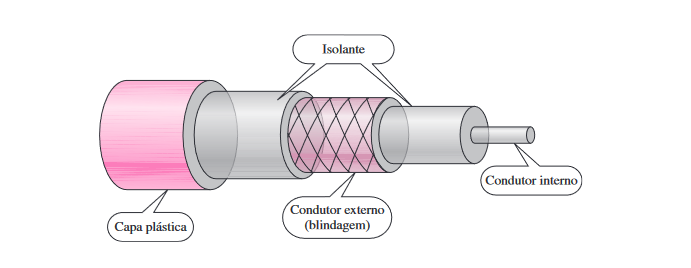
\includegraphics[width=15cm]{coaxial}
		\caption{cabo coaxial}
		\label{fig:coaxial}
	\end{figure}
	
	
	\subsubsection{Aplicações e mercado}
	O cabo coaxial dominou a industria durantes muito tempo, principalmente na área televisiva, sistemas de antena, redes de computadores e etc, mas ultimamente seu uso vem diminuindo por conta de tecnologias como a fibra óptica. Porém, em lugares onde não é possível ter acesso a internet com essas novas tecnologias, ele ainda é utilizado.
	
	\subsubsection{Vantagens}
	\begin{itemize}
		\item Longa transmissão: O cabo coaxial é capaz de transmitir dados a longas distâncias sem perder qualidade.
		\item Resistentes a interferências: São menos propensos a ter problemas com ruídos. e interferências.
		\item Durabilidade: É bem resistente a danos causados pelo ambiente.
	\end{itemize}
	\subsubsection{Desvantagens}
	\begin{itemize}
		\item Limitação de banda: Não é capaz de transmitir com tanta velocidade comparada, por exemplo, com fibra óptica.
		\item Dificuldade de instalação: Em comparação com outros cabos, ele é volumoso e rígido o que atrapalha sua instalação.
		
	\end{itemize}
	
	\subsection{Cabo trançado}
	Criado em 1880 por Alexander Graham Bell para resolver problemas causados por fios de cobre isolados que sofriam muito com problemas de interferência eletromagnética, fazia que a transmissão se tornasse incompreensível.
	
	É formado por dois condutores de cobre, revestido por material isolante de plástico. Eles são traçados juntos. Um dele é usado como terra de referência e o outro é onde transporta os sinais elétricos. O fio por ser trançado é menos suscetível a interferências e linha cruzada. 
	
\begin{figure}[H]
	\centering
	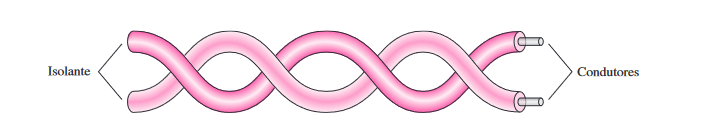
\includegraphics[width=15cm]{par-trançado}
	\caption{Par trançado}
	\label{fig:par-trancado}
\end{figure}
	
	\subsubsection{Blindados vs Não blindados}
	Há dois tipos de cabo: Blindado e Não blindado.
	
	Não blindado:  O cabo de par trançado não blindado (UTP) não há camada de blindagem, ele é mais flexível e fácil de instalar do que o STP. Geralmente é o mais utilizado para ambientes de baixa interferências eletromagnéticas.
	
	Blindado - O (STP) É composto por uma folha de metal que reveste cada par de condutores isolados. Faz com que a qualidade do cabo aumente, diminuindo ainda mais a penetração de interferências ou linha cruza, mas o deixa mais denso e caro. Usado para lugares com alta interferências eletromagnéticas.
	
	\begin{figure}[H]
		\centering
		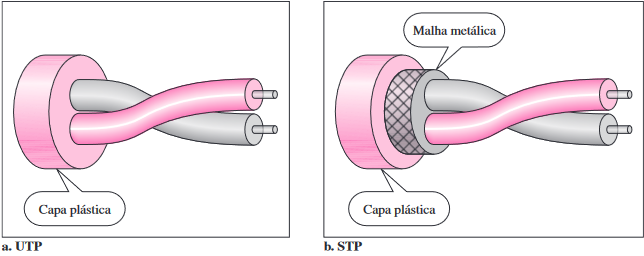
\includegraphics[width=15cm]{utpStp}
		\caption{UTP STP}
		\label{fig:utpstp}
	\end{figure}
	
	
	\subsubsection{Aplicações e mercado}
	O par trançado ainda é forte nos dias atuais, principalmente para utilizações em linhas telefônicas para transmissão de dados e voz, redes de computadores locais (LANs), sistemas de seguranças. Um dos principais é o seu custo e sua fácil instalação.
	
	\subsubsection{Vantagens}
	\begin{itemize}
		\item Custo-benefício: São mais baratos que as outras opções
		\item Fáceis de instalar: São bem simples de fazer a instalação.
		\item Alta velocidade: Em comparação ao cabo coaxial eles são bem mais rápidos
		\item Flexibilidade: Podem ser dobrador facilmente sem quebrar.
	\end{itemize}
	
	\subsubsection{Desvantagens}
	\begin{itemize}
		\item Limitações de distância: São limitados a poucas distâncias, no geral até 100 metros.
		\item Problema de segurança: Pode ser interceptado por um outra pessoa.
		\item Quebráveis: Por serem finos são fáceis de quebrar.
	\end{itemize}

	\subsection{Fibra óptica}
	A fibra óptica é baseada na capacidade que a luz possui de carregar informações, em um meio de vidro, por distâncias maiores do que sinais elétricos em cobre. O conceito de Fibra óptica já era conhecida na física, mas foi em 1970 que Dr. Robert Maurer, Donnald Keck e Peter Schultz criaram uma fibra com atenuação medida de menos de 20 dB por km, isso é,  ela possuía menor perda de sinal ao longo da distância percorrida. Isto a tornou a fibra óptica mais pura já criada na época.
	
	\subsubsection{Aplicações e mercado}
	É o meio de transmissão mais em alta no mercado. Ideal para quase todas as áreas: Internet, rede telefônica, televisão, sensores e cabos submarinos. Porém, possui suas limitações tais qual seu acesso a áreas rurais. 
	
	O cabo de fibra óptica reduz gasto de energia comparado com cabos coaxiais. Em 100 metros de distância, a fibra óptica consome apenas 1 watt em comparação ao cabo coaxial que gasta 3.5 watts. Não possuem cobre na sua estrutura, material conhecido pela sua extração ser perigosa ao ambiente.
	
	\subsubsection{Vantagens}
	\begin{itemize}
		\item Banda larga: Pode percorrer longas distâncias.
		\item Imune a interferências: Rádio e eletromagnéticas não afetam a fibra óptica.
		\item Leves: São muito mais leves do que cabos coaxial.
		\item Pouca perda de sinal: Dados viajam a longa distância sem precisar de amplificação.
		\item Seguros: Sem chances de causar curto.
	\end{itemize}
	
	\subsubsection{Desvantagens}
	\begin{itemize}
		\item Frágeis: São muito mais vulneráveis a danos do que outros cabos
		\item Caros: São caros de ser produzida devido ao custo dos materiais e mão de obra.
		\item Reparação: São difíceis de reparar e caro.
		\item Propagação unidirecional da luz: Se propaga em apenas uma direção.
	\end{itemize}
	
	\subsubsection{Como funciona}
	É baseado no princípio da física de reflexão interna total da luz. Segundo a teoria: "A luz reflete e refreta dependendo do ângulo em que atinge uma superfície". Portanto, a luz é movida até a outra extremidade do cabo sendo refletida dentro do núcleo que atua como o guia para a transmissão da luz.
	
	A fibra é feita com Núcleo, casca e revestimento primário. O núcleo é onde a luz viaja, a casca é uma proteção para evitar que a luz escape, ambos são feitos de vidro. O revestimento primário é feito de camadas de polímeros que protege o núcleo e a casca contra danos físicos. 
	
		
	\begin{figure}[H]
		\centering
		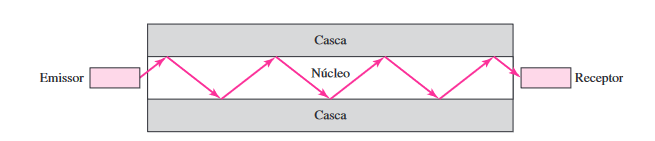
\includegraphics[width=15cm]{fibra-optica}
		\caption{Fibra óptica}
		\label{fig:fibra-optica}
	\end{figure}
	
	\subsubsection{Monomodo e multimodo}
	Há duas categorias de fibra óptica.
	
	As Multimodo são mais baratas de implementar, possuem um diâmetro maior no núcleo, uma casca mais fina e permite que vários feixes de luz navegam simultaneamente. O problema é que limita a largura de banda, pois terão propagação de luz em diferentes ângulos e direções. Geralmente é utilizado para pequenas distâncias.
	
	\begin{figure}[H]
		\centering
		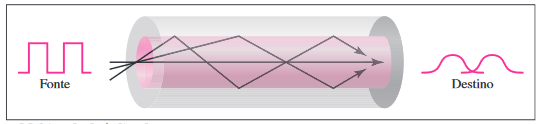
\includegraphics[width=15cm]{multimodo}
		\caption{Multimodo}
		\label{fig:multimodo}
	\end{figure}
	
	O monomodo possuem núcleo menor, uma casca mais grossa e apenas um feixe de luz se propagando por fibra. Com isso, mantem a integridade do sinal em longas distâncias. Seu custo é mais elevado e são mais difíceis de conectar. Geralmente usado para maiores distâncias.
	
	\begin{figure}[H]
		\centering
		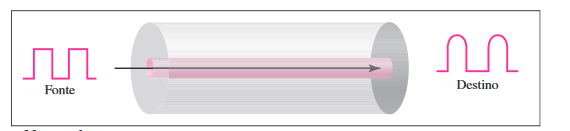
\includegraphics[width=15cm]{monomodo}
		\caption{Monomodo}
		\label{fig:monomodo}
	\end{figure}

\bibliographystyle{alpha}
\bibliography{telecom-ref}
	
\end{document}
